% Chandohasam: final paper (ACL format). Built on the mid-submission (Chandohasam__Towards_Semantically_Coherent_...pdf,
% 20 Oct 2026); plan, claim register and sources in FINAL_PLAN.md. Every number carries a "% src:" comment naming the
% file it comes from. Placeholders: \pend{...} in the text and \tbd in tables mark results of runs still in progress.
% Build: tectonic -X compile final.tex   (or xelatex + bibtex, as the Makefile does for main.tex).
\documentclass[11pt]{article}

\usepackage[final]{acl}

\usepackage{fontspec}
\setmainfont{texgyretermes}[Extension=.otf, UprightFont=*-regular, BoldFont=*-bold, ItalicFont=*-italic,
  BoldItalicFont=*-bolditalic]
\newfontfamily\telugufont{Noto Sans Telugu}[Script=Telugu, Scale=MatchLowercase]
\newcommand{\te}[1]{{\telugufont #1}}

\usepackage{microtype}
\usepackage{amsmath,amssymb}
\usepackage{graphicx}
\usepackage{booktabs}
\usepackage{tabularx}
\usepackage{makecell}
\usepackage{multirow}
\renewcommand{\theadfont}{\footnotesize}
\usepackage{enumitem}
\usepackage{float}
\usepackage{algorithm}
\usepackage{algpseudocode}
\usepackage{xcolor}
\usepackage{tikz}
\usetikzlibrary{positioning,arrows.meta}

\setlist{nosep, leftmargin=1.1em, labelsep=0.4em}
\newcolumntype{Y}{>{\raggedright\arraybackslash}X}
\renewcommand{\algorithmicrequire}{\textbf{Input:}}
\renewcommand{\algorithmicensure}{\textbf{Output:}}
\algnewcommand{\Symbols}{\item[\textbf{Symbols:}]}
\makeatletter
\algnewcommand{\LongState}[1]{\State\parbox[t]{\dimexpr\linewidth-\ALG@thistlm-1pt\relax}{#1\strut}}
\makeatother
\algrenewcommand\algorithmicindent{0.8em}
\algrenewcommand\alglinenumber[1]{\tiny #1:}
\newcommand{\U}{\textsc{u}}
\newcommand{\I}{\textsc{i}}
% placeholders for results of runs still in progress (FINAL_PLAN.md §5 lists each one and its ETA)
\definecolor{pend}{HTML}{B03A2E}
\newcommand{\pend}[1]{\textcolor{pend}{\textsf{\footnotesize[pending: #1]}}}
\newcommand{\tbd}{\textcolor{pend}{\textsf{tbd}}}
\newcommand{\sig}{$^{\ast}$}
% generated table rows (analysis/make_grid_tables.py); the primitive \input stays expandable inside a tabular
\makeatletter\newcommand{\rowsfrom}[1]{\@@input #1 }\makeatother
\hyphenpenalty=1000
\emergencystretch=2em

\title{Chandohasam: Towards Semantically Coherent Telugu Metrical Poetry Generation with Text Diffusion}

\author{
 \textbf{Samvaran Kashyap Rallabandi},
 \textbf{Mahesh Emani},
 \textbf{Radhe Shyam Salopanthula}
\\
 IIIT Hyderabad
\\
 \small{\{samvaran.rallabandi, mahesh.emani, radheshyam.s\}@research.iiit.ac.in}
}

\begin{document}
\maketitle

\begin{abstract}
Telugu metrical poetry (\textit{padyaṃ}) must satisfy hard constraints on syllable weight (\textit{gaṇa}),
caesura (\textit{yati}) and line-initial rhyme (\textit{prāsa}) while conveying a given meaning
(\textit{bhāvaṃ}). We argue that the two halves of the task need different machinery: metre is decidable and
should be enforced exactly while decoding, whereas meaning must be learned from meaning-to-poem supervision.
Chandohasam compiles 37 metres into a minimal labelled automaton (DAWG) and enforces gaṇa, yati and prāsa
jointly inside the decoding loop of autoregressive, encoder--decoder, block-diffusion and masked-diffusion
generators. On 100 held-out prompts whose source poems are part of our human study, no fine-tuned model graded so
far writes more than 8\% of its poems in metre unaided (the source poems pass the same strict check half the
time). The controller puts 99--100\% in metre at a cost of 4--14 points of attested words, and two lexical layers
added to it (attested syllables and words) remove most of that cost: the fine-tuned models then keep 79--85\%
attested words, and our 523M syllable-level masked diffusion model, pretrained on Telugu and fine-tuned on 300k
crawled poems, matches the source poems (85.4\% against 85.7\%). Left-to-right models learn more of the metre
unaided; the diffusion models keep more words and topic under the constraint, at the price of more one-syllable
filler. Scaling within a model family brought no significant gain, and reinforcement learning with our
deterministic metrics as verifiable rewards did not make metre the default and degraded the diffusion model. In
a five-annotator human study, three annotators agree fairly to moderately ($\alpha$ 0.33--0.48) and rate
Gemini's poems easier to read but less faithful and less poetic than the poets'; measuring meaning remains the
open problem. We release the benchmark, controller, evaluation suite and ratings.
\end{abstract}

\section{Introduction}\label{sec:intro}

A poem must convey coherent ideas and also satisfy constraints of rhythm, rhyme and ornament. The Telugu
\textit{padyaṃ} is strict: every line follows a syllable-weight pattern (\textit{gaṇa}), an akṣara at the
caesura agrees in sound with the line's first akṣara (\textit{yati}), and the second akṣara of every line
repeats the consonant of the first line's (\textit{prāsa}). Good verse also carries figures of sound
(\textit{śabdālaṅkāra}) and sense (\textit{arthālaṅkāra}); the \textit{Kāvyālaṅkārasaṅgrahamu}
\citep{ramarajabhushana_kas1920} asks for \textit{śabdārtha samanvaya}, the balance of sound and sense, through
\textit{anuprāsa} (alliteration), \textit{mādhurya} (euphony), \textit{ojas} (density) and \textit{prasāda}
(clarity).

\paragraph{Form and sense are different problems.} Whether a poem is in a metre is \emph{decidable}: each
metre's set of legal lines is finite (370,315 for our 37 metres), so validity can be checked exactly and
enforced while decoding. Whether a poem says what it was asked to say is not, and has to be learned and
measured. Prior systems either learn form and keep only part of it, or impose it and lose meaning: Sanskrit
constrained decoding reaches near-perfect metre while raters score coherence at 2.1--2.7 out of 5
\citep{jagadeeshan2026chandomitra,jagadeeshan2026pingala}. Our premise: enforce exactly what is decidable,
learn the rest from supervision, and measure it without over-claiming. We ask:
\textbf{RQ1} Can metre be guaranteed for any generator, and at what cost?
\textbf{RQ2} Does meaning-to-poem supervision reduce that cost, and which architecture and scale benefit most?
\textbf{RQ3} Can reinforcement learning with verifiable rewards (RLVR) from deterministic metrics make metre
the default? \textbf{RQ4} How far can the meaning of a generated padyaṃ be measured?

\paragraph{Contributions.}
(1)~A benchmark of 12,673 labelled poems from four sources with prose meanings, and a deterministic metrical
controller (a 1,431-state DAWG with yati and prāsa engines) that identifies 7,355 of the 7,365 Bhāgavatamu poems
in catalogue metres and none as a wrong metre. (2)~A grid of nine generators (four architectures,
120M--26B parameters), untuned or fine-tuned, free or constrained, with paired tests.
(3)~The finding that supervision plus exact enforcement is what works: under the constraint, fine-tuning
raises attested words from 34--60\% to 73--78\%, two lexical layers to 79--85\%, where our best diffusion model
matches the source poems; scale did not substitute for supervision. (4)~A negative RLVR result with an account of why deterministic metrics
fail as rewards, especially for masked diffusion. (5)~An evaluation suite, a human study with an agreement
and drift analysis, and an LLM-judge protocol.

\section{Related Work}\label{sec:related}

\paragraph{Poetic form.} The \emph{soft route} steers a model toward the form and discards failures:
Deep-speare learns metre with language for English sonnets \citep{lau2018deepspeare}, SongNet encodes rigid
SongCi formats \citep{li2020songnet}, and PoeLM generates from length and rhyme codes and keeps candidates that
pass scansion \citep{ormazabal2022poelm}, a recipe carried to Bangla, whose authors report semantic drift when
several codes apply at once \citep{amina2025}. These constraints are aggregates (a mātrā total, an end rhyme).
The \emph{hard route} guarantees form while decoding \citep{ghazvininejad2016,lu2021neurologic,geng2023grammar};
Chandomitra and PINGALA reach near-perfect Anuṣṭubh this way, with the coherence scores quoted above.
PoetryDiffusion targets semantics and metre together with Diffusion-LM and a learned metrical classifier
\citep{hu2024poetrydiffusion,li2022diffusionlm}. We keep a deterministic controller inside the decoding loop
and learn meaning from supervision.

\paragraph{Diffusion language models.} Discrete diffusion \citep{austin2021d3pm} led to masked diffusion
language models \citep{sahoo2024mdlm}, block diffusion that interpolates with autoregression
\citep{arriola2025block}, and large diffusion LMs \citep{nie2025llada}. A diffusion model sees both
neighbours of a position, which suits constraints that bind distant akṣaras (yati, prāsa).

\paragraph{Learning from verifiable rewards.} Expert iteration fine-tunes a model on its own best samples
\citep{anthony2017exit,zelikman2022star,gulcehre2023rest}; GRPO and RLVR optimise programmatic rewards
directly \citep{shao2024deepseekmath,lambert2024tulu3}, and for diffusion models need likelihood surrogates
\citep{zhao2025d1}. Optimising a proxy over-fits it \citep{gao2023overoptimization}, and training on
self-generated data narrows the distribution \citep{shumailov2024collapse}.

\paragraph{Evaluation.} Metre identification is solved deterministically for Sanskrit \citep{terdalkar2023}
and approximately for Telugu \citep{boddu2025chandassu}; meaning has no such checker. Sound figures have
deterministic identifiers for Sanskrit \citep{barbadikar2023yamaka,barbadikar2024anuprasa} and simile
identification has begun \citep{jadhav2025upama}; Telugu's alpha-syllabary lets us adapt the former, while
arthālaṅkāras stay out of scope. MAUVE compares text distributions \citep{pillutla2021mauve}; LLM judges
are used for open-ended text \citep{zheng2023judge,liu2023geval}; and human raters of creative text agree
little, so correlation is advocated beside agreement \citep{amidei2019agreement,karpinska2021perils}.

\section{Benchmark and Data}\label{sec:data}

\paragraph{Benchmark.} We source Telugu padyaṃs from Pothana's \textit{Āndhra Mahābhāgavatamu}, from an online
compilation with word glosses and meanings \citep{pothana15c}; Vemana's \textit{śatakaṃ}; Kuchimanchi
Timmakavi's \textit{acca tĕlugu} Rāmāyaṇamu and three śatakas; and the Chandassu dataset
\citep{boddu2025chandassu,boddu2025kaggle} (Table~\ref{tab:benchmark}). The Bhāgavatamu is the gold set,
with edition meanings and glosses; the other meanings are LLM-generated, and every English meaning is a
machine translation of the Telugu bhāvaṃ. Sanity metrics (Appendix Table~\ref{tab:sanity}) show that a
length-ratio gate separates real from shuffled poem--meaning pairs in three files (96--98\% against
62--67\%) but not in Vemana, whose machine meanings have uniform length (84.5\% against 82.6\%); LaBSE
\citep{feng2022labse} ranks the correct pairing above a shuffled one with AUC 0.85--0.94. Verbatim
duplication is negligible (13 near-duplicate pairs among the 12,704 verse poems, of which 12,673 carry a metre
label; 31 Kuchimanchi poems have none); the remaining repetition is formulaic
(refrains recur in 77.1\% of Vemana's poems, raising its Yule's K to 99.9 against 1.4--4.1 elsewhere), so
splits keep works together. A subword tokenizer spends 1.2--1.4 tokens per akṣara, which motivates our
syllable-level tokenizer.
% src: mid-submission Tables 1-2 (data_sanity_metrics/data_sanity_metrics_report.md)

\begin{table*}[t]
\centering\footnotesize
\begin{tabular}{@{}lrrrrr@{}}
\toprule
rule, labelled verse poems & Bhāgavatamu & Vemana & Kuchimanchi & Chandassu & total \\
\midrule
poems & 7,366 & 1,164 & 1,611 & 2,532 & 12,673 \\
1. gaṇa & 99.85\% & 87.2\% & 96.5\% & 85.0\% & 95.3\% \\
2. prāsa, relaxed (strict) & 99.8\% (96.7\%) & 95.6\% (93.4\%) & 99.9\% (97.7\%) & 98.8\% (93.7\%) & 99.2\% (95.9\%) \\
3. yati, relaxed (strict) & 91.4\% (90.7\%) & 96.4\% (95.7\%) & 93.9\% (92.9\%) & 87.9\% (86.6\%) & 91.5\% (90.6\%) \\
\bottomrule
\end{tabular}
\caption{The benchmark: 12,673 labelled poems, and the share valid under each rule of our engines (relaxed
profile; strict in brackets). The whole benchmark is held out from fine-tuning.}
\label{tab:benchmark}
\end{table*}


\paragraph{Fine-tuning corpus.} We crawled over 300k Telugu poems with their prose meanings from the
internet. After removing every poem of the four benchmark works, 365,680 poems remain; the 300,763 that have
an engine-confirmed metre and a meaning form the fine-tuning pool (one \emph{pass} = one epoch over it).
% src: diffusion_finetuning/data/e6/DATA_CARD.md; report.md §2.1

\paragraph{Evaluation prompts.} Validation draws 906 Bhāgavatamu poems (skandhas 1, 2 and 7), of which 114
in 11 metres form \textbf{val-114}, used for model selection and the diffusion, decoder and RL comparisons. The
other 10,749 benchmark poems are the test pool. \textbf{The grid} takes 100 of them in 25 metres that are also
poems of our human-evaluation pool (Bhāgavatamu 50, Vemana 20, Kuchimanchi 20), plus 10 of the pool's
Gemini-generated poems, so every grid prompt has a human-rated poem on the same bhāvaṃ (56 rated in phase 1,
44 to come). Gemma-4 26B-A4B \citep{gemma4_2026} retells each human bhāvaṃ in new words and order under six
checks (App.~\ref{app:prompts}), so a model cannot score by recalling a pair it may have seen; Gemini's
bhāvaṃs are used as written. The 112 test poems found in the MDLMs' pretraining text are excluded throughout;
splits count records in which a sīsamu and its closing gīti are one poem (11,655 records).
% src: report.md §2.1-2.2; full_grid_experiments/prompts/summary.json

\section{The Chandohasam Framework}\label{sec:framework}

In Figure~\ref{fig:framework}, a deterministic controller guarantees structure while decoding, a generator
fine-tuned on meaning-to-poem pairs chooses the words, a separate evaluation suite measures what validity does
not, and an optional RLVR stage feeds rewarded samples back into training.

\begin{figure}[t]
\centering
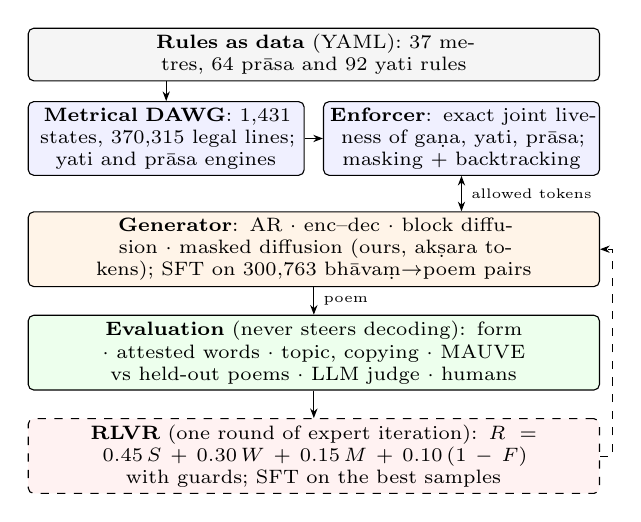
\begin{tikzpicture}[font=\scriptsize, >={Stealth[length=3.5pt]},
  box/.style={draw, rounded corners=2pt, align=center, inner sep=2.2pt, text width=#1}, box/.default=7.1cm]
\node[box, fill=gray!8] (rules) {\textbf{Rules as data} (YAML): 37 metres, 64 prāsa and 92 yati rules};
\node[box=3.35cm, fill=blue!6, below=2.5mm of rules.south west, anchor=north west] (dawg) {\textbf{Metrical
DAWG}: 1,431 states, 370,315 legal lines; yati and prāsa engines};
\node[box=3.35cm, fill=blue!6, below=2.5mm of rules.south east, anchor=north east] (enf) {\textbf{Enforcer}:
exact joint liveness of gaṇa, yati, prāsa; masking + backtracking};
\node[box, fill=orange!9, below=4.5mm of dawg.south west, anchor=north west] (gen) {\textbf{Generator}: AR
$\cdot$ enc--dec $\cdot$ block diffusion $\cdot$ masked diffusion (ours, akṣara tokens); SFT on 300,763
bhāvaṃ$\to$poem pairs};
\node[box, fill=green!7, below=3.5mm of gen] (eval) {\textbf{Evaluation} (never steers decoding): form $\cdot$
attested words $\cdot$ topic, copying $\cdot$ MAUVE vs held-out poems $\cdot$ LLM judge $\cdot$ humans};
\node[box, fill=red!5, dashed, below=3.5mm of eval] (rl) {\textbf{RLVR} (one round of expert iteration):
$R = 0.45\,S + 0.30\,W + 0.15\,M + 0.10\,(1-F)$ with guards; SFT on the best samples};
\draw[->] (rules.south -| dawg) -- (dawg);
\draw[->] (dawg) -- (enf);
\draw[<->] (enf.south) -- node[right, font=\tiny]{allowed tokens} (enf.south |- gen.north);
\draw[->] (gen) -- node[right, font=\tiny]{poem} (eval);
\draw[->] (eval) -- (rl);
\draw[->, dashed] (rl.east) -- ++(1.6mm,0) |- (gen.east);
\end{tikzpicture}
\caption{The Chandohasam framework. Validity is decided by the controller inside the decoding loop; meaning is
left to the fine-tuned generator and measured separately.}
\label{fig:framework}
\end{figure}

\subsection{Metrical controller}\label{sec:controller}

The controller reads YAML specifications of 37 metres and their gaṇa classes, with 64 prāsa and 92 yati rules
from Appakavi's \textit{Appakavīyaṃ} \citep{appakavi1656} (Appendix Table~\ref{tab:metres}). Each metre is a
prosodic grammar (poem $\to$ lines $\to$ gaṇa classes $\to$ gaṇas $\to$ guru/laghu, \U/\I); the grammars are
flattened into one right-linear grammar, determinised, and minimised into a labelled DAWG of 1,431 states
whose accepting states carry their metre and slot (Algorithm~\ref{alg:build}; \citealp{daciuk2000}). It
accepts exactly the 370,315 legal lines and is built in under half a second. Figure~\ref{fig:dawg}
illustrates the construction. The controller answers three queries: \texttt{identify} walks a poem's
scansion lattice and returns every accepting metre and slot, with the point at which each rejected metre
became impossible; \texttt{viable\_prefix} and \texttt{next\_symbols} return the weights that can still
complete a slot; \texttt{segment} returns gaṇa divisions and yati seats. Of the 7,366 labelled Bhāgavatamu
poems, 7,365 are in catalogue metres (one is a ślokamu); the controller identifies 7,355 of them with their
labelled metre, none as a wrong metre, and leaves 10 unclassified.

\begin{figure}[t]
\centering
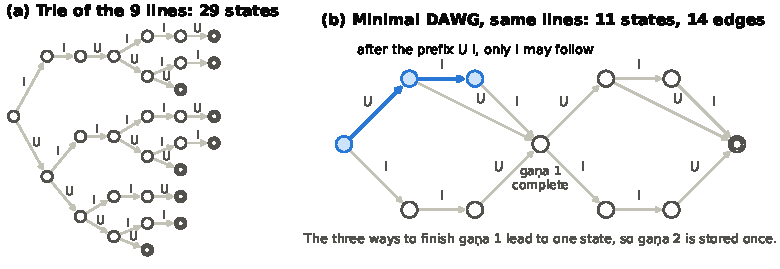
\includegraphics[width=\columnwidth]{figures/fig2_dawg_two_panel.pdf}
\caption{The DAWG on a toy slot of two gaṇas, each \U\U, \I\I\U\ or \U\I\I: (a) the trie of its 9 legal lines
has 29 states; (b) merging states with equal futures leaves 11 states and 14 edges. After the prefix \U\I,
only \I\ may follow: the query the decoder asks.}
\label{fig:dawg}
\end{figure}

\subsection{Constrained decoding}\label{sec:decoding}

The decoder uses the DAWG as a hard constraint, not a post-hoc filter. The enforcer keeps the live automaton
states with prāsa and yati registers (Algorithm~\ref{alg:step}); a token is allowed only if, after all its
akṣaras, some completion of the metre still satisfies gaṇa, prāsa and yati. An akṣara's weight stays pending
until the next onset is known, since a following conjunct makes it heavy. Because liveness is exact, a valid
path never reaches a dead end. Three strategies use the mask (Algorithm~\ref{alg:decode}): \emph{masking
only}; \emph{masking + backtracking}, which saves checkpoints and rewinds, with a raised temperature, when the
allowed set or its mass collapses; and \emph{hybrid}, which re-ranks allowed tokens toward completing the
line. Sampling uses temperature 0.7 and top-$p$ 0.9. On diffusion canvases the model's proposals are
committed left to right while each is allowed and confident; otherwise the strategy chooses at the first open
position, and a backtrack returns positions to noise. A NaN in this confidence test (fixed 21 October) affects
only the September DiffusionGemma grid (Appendix Table~\ref{tab:sept}; not rerun).

In the September grids all 4,995 constrained poems, and 555 of 555 with random logits, are in metre. On the grid,
with masking + backtracking, 0--1\% of fine-tuned models' poems and 7--15\% of the pretrained-only MDLMs' fail the
strict check after decoding (counted as failures; cause not yet traced). The \emph{v2} decoder adds a hard inventory
of 6,131 akṣaras attested in $\geq$ 3 training poems (A) and a soft bias toward 212,422 attested words (B),
keeping exactness; with it no grid poem fails.
% src: report.md §4.1, §4.4; full_grid_experiments/results/grid.md

\subsection{Generators}\label{sec:models}

Table~\ref{tab:models} lists the generators. The Gemma-4 instruction models E4B and 26B-A4B \citep{gemma4_2026} are prompted
zero-shot with the metre's rules and the topic. All others get supervised fine-tuning (SFT) on one task,
metre + bhāvaṃ $\to$ poem, with the loss on the poem only; we do no instruction tuning.
\textbf{Nandi-Mini-150M} \citep{hf_nandi150m} is a byte-BPE autoregressive model. \textbf{T5Gemma 2}
\citep{t5gemma2_2025} is an encoder--decoder whose encoder also reads the metre's rules; 15\% of its examples
ask for a poem's scansion. \textbf{DiffusionGemma 26B-A4B} \citep{hf_diffusiongemma} is a block-diffusion
mixture-of-experts model, adapted with LoRA \citep{hu2022lora} in its chat format. Our \textbf{Chandohasam
MDLMs} are masked diffusion LMs \citep{sahoo2024mdlm} with one token per akṣara (\S\ref{sec:pretraining}),
fine-tuned in three stages: continued pretraining on poem + meaning documents with 15\% prose replay;
multi-task SFT (meaning $\to$ poem 50\%, poem $\to$ meaning 15\%, repair 15\%, metre $\to$ poem 10\%,
glosses 10\%); and a final meaning $\to$ poem phase.
% src: report.md §3.1-3.6

\begin{table}[t]
\centering\scriptsize\setlength{\tabcolsep}{2.4pt}
\begin{tabular}{@{}llllr@{}}
\toprule
model & arch. & tokens & trained (params) & passes \\
\midrule
Gemma-4 E4B/26B & AR, IT & subword & none & -- \\
Nandi-Mini-150M & AR & byte BPE & full (153M) & 3.5 \\
T5Gemma 2 270M/1B & enc--dec & subword & full (0.8B/1.7B) & 1 \\
T5Gemma 2 4B & enc--dec & subword & LoRA r128 (477M) & 0.16/1 \\
DiffusionGemma 26B & block diff. & subword & LoRA r16 (11.5M) & 1 \\
MDLM-120M (ours) & masked diff. & akṣara & full (120M) & $\approx$3.5 \\
MDLM-523M (ours) & masked diff. & akṣara & full (523M) & $\approx$3.5 \\
\bottomrule
\end{tabular}
\caption{Generators. \emph{Passes}: epochs over the 300,763-poem pool (T5Gemma 4B: also its snapshot after 48k
examples, 0.16). The 270M count includes its vision tower.}
\label{tab:models}
\end{table}

\subsection{Pretraining our masked diffusion models}\label{sec:pretraining}

MDLM-120M is a bidirectional transformer (12 layers, width 768, RoPE, SwiGLU) trained from scratch as a masked
diffusion language model \citep{sahoo2024mdlm} on 4.98B tokens of Telugu from Sangraha
\citep{khan2024indicllmsuite}, IndicCorp v2 \citep{doddapaneni2023indiccorp} and Wikipedia
\citep{wikimedia2023telugu}, on one 8\,GB laptop GPU in 2 days 19 hours, after removing every document that
shares a 20-token window with any of $\approx$767k poems. MDLM-523M (16 layers, width 1,536) is grown from it
function-preservingly and trained to 10.49B tokens. The tokenizer has 45,591 tokens, 44,835 of them whole
akṣaras; BPE never merges across akṣaras (1.002 tokens per akṣara on the Bhāgavatamu), so the constraint acts
on single syllables. Generation fills a 512-token canvas with the prompt fields unmasked.
% src: report.md §3.3; mid-submission §4.4

\subsection{Evaluation suite}\label{sec:eval}

Measures are computed per poem, identically for every model and for the source (\emph{gold}) poems.
\textbf{In metre}: all lines accepted under canonical scansion (no pāda-final guru, no optional weight before a
conjunct), strict prāsa and yati without sandhi, exactly the decoder's rules. Poets do not write to them (the
grid's gold poems pass 50.0\%), so for free text the fairer measures are
\textbf{vṛtta lines on pattern} (lines whose weights, last akṣara free, match the gold poem's) and the chandas
skill $S = 1 - r/r_{\mathrm{chance}}$, $r$ the edit rate to the nearest valid poem (Algorithm~\ref{alg:chandas}).
\textbf{Real words}: the share of 2+-akṣara words attested in the training lexicon, allowing sandhi-softened
onsets and compounds; akṣaras shuffled across same-length words of the 10,749 test poems score 19.9\% (51.5\%
for two-akṣara words) against 89.6\% for the poems, so it is a lower bound on valid Telugu and a soft upper
bound on noise. \textbf{One-akṣara}: single-syllable words (filler). \textbf{Recognised}: LaBSE ranks the
poem's own prompt above 9 others (chance 10\%), a topic signal. \textbf{Copy}: words found in the prompt. \textbf{MAUVE} \citep{pillutla2021mauve} embeds poems
with EmbeddingGemma 2 \citep{hf_embeddinggemma2} and compares each set with the held-out benchmark poems
written for the same prompts (5 seeds; signs Gemma's tokenizer cannot write are stripped everywhere). Differences are paired bootstrap tests over prompts
\citep{efron1993bootstrap} (10,000 resamples) and exact McNemar tests \citep{mcnemar1947}; \sig\ marks a 95\%
interval that excludes 0. The poetics suite (Appendix Table~\ref{tab:metrics}) is reported for the untuned
grid only.
% src: report.md §2.3, §5.9; metrics/mauve_padyarchana/report_more_stripped.md


\paragraph{LLM judge.} \pend{not run} A judge model, never a generator or a reward, rates every grid poem on the
human rubric's 1--5 scales \citep{zheng2023judge,liu2023geval}, admitted only after a validation against the
human ratings (App.~\ref{app:judge}).

\subsection{RLVR}\label{sec:rlvr-method}

We ran one round of reward-filtered expert iteration \citep{anthony2017exit,gulcehre2023rest}: 2,188 training
prompts in the 11 val-114 metres, 8 free samples each; the best sample per prompt, then the top half, mixed
1:1 with real poems, fine-tuned with each model's own SFT loss. The reward
$R = 0.45\,S + 0.30\,W + 0.15\,M + 0.10\,(1 - F)$ combines chandas skill $S$, real words $W$, recognition $M$
(counted only if copy $\leq$ 10\%) and filler excess $F$, and is zeroed for an empty poem, a repeated line, a
training line or copy above 18\%. It passed its gate: gold poems score 0.877, above every model's free poems;
shuffled gold 0.190; the bhāvaṃ cut into lines 0.000. Success was fixed in advance: skill $+0.05$ (or,
for Nandi, $+5$ points of poems in metre), real words down and filler up by at most 1 point, copy $\leq$ 5\%,
no memorisation, and a distribution guard.
% src: RL/PLAN.md §5; RL/results/reward_gate.md

\section{Results}\label{sec:results}

\subsection{RQ1: form is guaranteed, not learned}\label{sec:rq1}

Without the controller no model writes in metre: untuned Gemma-4 E4B, 26B-A4B and DiffusionGemma write 0 of 555
poems each in metre, against 555 of 555 constrained (App. Table~\ref{tab:sept}), and on the grid the best
fine-tuned free cell reaches 8.0\%, against 50.0\% for the source poems under the same strict check
(Table~\ref{tab:grid-free}). Constrained, 99--100\% of the fine-tuned and 85--100\% of the untuned models' poems
are in metre, and with the v2 layers all are (Table~\ref{tab:grid}). Form comes from the decoder; its cost is
lexical. Untuned models keep 33.5--59.6\% real words, and with masking + backtracking alone the fine-tuned ones
lose 4.2--13.9 points against their own free poems (all \sig), most at yati seats (on val-114 with masking only,
MDLM-523M keeps 0.39 of its probability there and has its first choice overridden 58\% of the time).
% src: tables/grid_*_rows.tex; full_grid_experiments/results/grid.json (tests); report.md §5.2

\begin{table}[t]
\centering\scriptsize\setlength{\tabcolsep}{2.2pt}
\begin{tabular}{@{}llrrrrr@{}}
\toprule
model & train & \makecell[r]{in\\metre} & \makecell[r]{vṛtta\\lines} & \makecell[r]{real\\words} & recog. & MAUVE \\
\midrule
\rowsfrom{tables/grid_free_rows.tex}
\bottomrule
\end{tabular}
\caption{The grid, \textbf{free} generation: 100 held-out prompts, one poem each (\%). Groups: autoregressive,
encoder--decoder, block diffusion, masked diffusion (ours). Bracketed words: untuned models write prose. MAUVE:
against the 90 human gold poems (gold row: the human ceiling, \S\ref{sec:rq4}). \tbd: running \pend{Oct 30}.}
\label{tab:grid-free}
\end{table}

\begin{table*}[t]
\centering\scriptsize\setlength{\tabcolsep}{2.9pt}
\begin{tabular}{@{}ll|rrrrrr|rrrrrr|r@{}}
\toprule
 & & \multicolumn{6}{c|}{v1: masking + backtracking} & \multicolumn{6}{c|}{v2: + attested akṣaras (A) and words (B)} & \\
model & train & metre & words & 1-akṣ. & rep. & recog. & MAUVE & metre & words & 1-akṣ. & rep. & recog. & MAUVE & judge \\
\midrule
\rowsfrom{tables/grid_constr_rows.tex}
\bottomrule
\end{tabular}
\caption{The grid, \textbf{constrained} (100 prompts, one poem each, \%; gold: the source poems as written):
in metre, real words, one-akṣara words, poems repeating a line, recognised, and MAUVE against the 90 human golds.
\tbd: running (DiffGemma LoRA; the v2 cells of Gemma-4 26B and DiffGemma \pend{Oct 30}) or not built (judge).}
\label{tab:grid}
\end{table*}

\subsection{RQ2: supervision, architecture and scale}\label{sec:rq2}

\paragraph{Supervision makes the constrained poems usable.} Under the constraint, SFT adds 18--36 points of real
words and 14--58 of recognition over the same model untuned (all \sig), and 7 and 14 points of in-metre poems for
the MDLMs; unaided, it adds 7--8 points in metre for T5Gemma (McNemar $p \leq 0.016$), 5 for Nandi ($p = 0.06$)
and none for the MDLMs. Nothing is copied: no fine-tuned grid poem shares a 12-akṣara run with its source poem or
a line with a training poem, nor (val-114 and test runs) a 12-akṣara run with any training poem.
% src: full_grid_experiments/results/grid.json (tests "ft vs base")

\paragraph{Architecture: order learns form, diffusion keeps words.} Unaided, Nandi and T5Gemma 270M put 37.8 and
38.8 more points of vṛtta lines on pattern than MDLM-523M but write 8.6 and 9.5 fewer real words (all \sig;
Table~\ref{tab:xmodel}). The controller supplies what the diffusion models lack: under it the MDLMs keep more real
words than Nandi (+4.7 with v1, +6.3 with v2, \sig) and as many as T5Gemma (+2.3 to +3.4, n.s.), and MDLM-523M is
recognised more often than T5Gemma 270M (+13.0, \sig). The price is filler: 5.4--6.2 points more one-akṣara words
than T5Gemma with v1 (\sig), 2.1 with v2 -- plausibly because a mask that removes a syllable, not a subword, lets
the model finish its word but pads a stuck line with syllables. These are comparisons of recipes: T5Gemma reads
the rules, and the MDLMs had continued pretraining and $\approx$3.5 passes against 1.

\begin{table}[t]
\centering\scriptsize\setlength{\tabcolsep}{2.6pt}
\begin{tabular}{@{}lrrrr@{}}
\toprule
B $-$ A (grid, paired) & vṛtta lines & words & one-akṣ. & recog. \\
\midrule
\rowsfrom{tables/xmodel_rows.tex}
\bottomrule
\end{tabular}
\caption{Paired differences on the 100 grid prompts (points; fine-tuned models; bootstrap over prompts; intervals
in \texttt{analysis/cross\_model\_tests.md}).}
\label{tab:xmodel}
\end{table}

\paragraph{Scale did not substitute for supervision.} Within a family, size changed nothing significant under the
constraint (MDLM 523M against 120M, T5Gemma 1B against 270M and 4B against 1B: real words $-$1.4 to $-$0.2, n.s.);
unaided, MDLM-523M learned more of the pattern than the 120M (+19.1 points of lines, \sig) but not whole poems.
Untuned DiffusionGemma 26B-A4B keeps only 33.5\% real words constrained; its whole-pool adapter is \pend{Oct 30}.

\subsection{Reducing the cost of the constraint}\label{sec:cost}

\paragraph{Lexical layers.} The v2 layers (A, B; \S\ref{sec:decoding}) raise real words by 3.9--8.1 points on the
fine-tuned rows and 7.1--13.1 on the untuned ones (all \sig) and put every pretrained-MDLM poem in metre. The
constraint then costs the autoregressive and T5Gemma models no measurable words against their own free poems
($-$1.3 to +3.4, n.s.) and MDLM-523M 3.6 points (\sig), whose 85.4\% real words equal the source poems' 85.7\%
($-$0.4, n.s.). Layer B prefers the lexicon the measure reads, so part of the gain is by construction; on val-114 it
held on an independent held-out lexicon (+9.7 for T5Gemma 1B, against +4.3 on the measure). Costs: more repeated
lines for untuned models (Gemma-4 E4B 6 $\to$ 17\%, MDLM-523M 13 $\to$ 39\%; fine-tuned rows 0--3\%) and 10 points
less recognition for MDLM-120M (\sig).
% src: full_grid_experiments/results/grid.json (tests "v2 A+B vs v1"); analysis/cross_model_tests.md; report.md §5.5

\paragraph{Backtracking and writing order.} On the four rows of the earlier 183-prompt grid run with all three
strategies, masking + backtracking is never significantly worse on words (Table~\ref{tab:strategies}); without it
a stuck decoder pads lines with one-akṣara words, and hybrid helps only an untuned model reach the metre. On
val-114 it has the highest log-probability and fewest overrides (MDLM-523M: $-$1.52 against $-$2.34 nats per token,
12\% against 24\%). Writing in any order, our
adaptation of PoetryDiffusion's whole-poem view \citep{hu2024poetrydiffusion}, did not help: with the metre exact,
blocks of 24 akṣaras raised real words by only 2.2--6.8 points but filler by 6.6--11.5, and left-to-right
backtracking beat every any-order arm.

\begin{table}[t]
\centering\scriptsize\setlength{\tabcolsep}{2.8pt}
\begin{tabular}{@{}llrrr@{}}
\toprule
row & measure & backtracking & masking only & hybrid \\
\midrule
MDLM-523M SFT & real words & 77.6 & $-$6.1\sig & $-$6.1\sig \\
 & one-akṣara & 10.2 & +6.9\sig & +0.8 \\
Nandi SFT & real words & 71.7 & $-$2.5\sig & $-$1.5 \\
MDLM-523M pretr. & in metre & 83.1 & +4.4 & +10.9\sig \\
 & repeats a line & 18.6 & +12.6\sig & $-$0.5 \\
 & one-akṣara & 18.7 & +1.2 & $-$6.7\sig \\
Nandi untuned & in metre & 100 & $-$2.2\sig & $-$3.3\sig \\
 & one-akṣara & 18.2 & +6.2\sig & +5.2\sig \\
\bottomrule
\end{tabular}
\caption{Strategies on the earlier 183-prompt grid: backtracking's value and each alternative's paired difference
(\sig: bootstrap; for Nandi's in-metre row the exact McNemar test gives $p$ = 0.125 and 0.031).}
\label{tab:strategies}
\end{table}
% src: report.md §5.4 (183-prompt grid, 2026-10-27)

\subsection{RQ3: why RLVR with deterministic rewards failed}\label{sec:rq3}

No trial met its criterion (Table~\ref{tab:rl}). For MDLM-120M, skill fell by 0.069 and vṛtta lines by 2.9
points while words rose by 3.8: the model became more fluent and less metrical. Distilling the constrained
decoder's poems instead was worse (skill $-$0.352). Nandi was nearly unchanged. Five properties, each visible
in the logs, explain it.

\begin{table}[t]
\centering\scriptsize\setlength{\tabcolsep}{1.1pt}
\begin{tabular}{@{}lrrrrrrr@{}}
\toprule
trial & \makecell[r]{any of 8\\in metre} & skill & lines & words & recog. & NLL & MAUVE \\
\midrule
MDLM-120M & 0.0 & $-$0.069\sig & $-$2.9\sig & +3.8\sig & $-$5.3\sig & +0.071 & $-$0.065 \\
MDLM-120M dist. & 0.0 & $-$0.352\sig & +2.7\sig & +1.4\sig & $-$4.6\sig & +0.079 & $-$0.119 \\
Nandi & 33.3 & $-$0.005 & $-$3.7\sig & +0.6 & +2.3 & +0.410 & 0.000 \\
Nandi, metre$^\dagger$ & 33.3 & $-$0.002 & $-$1.5 & +1.1\sig & +3.6\sig & +0.108 & $-$0.011 \\
\bottomrule
\end{tabular}
\caption{Expert iteration, after $-$ before on free poems (val-114, 8 per prompt). \emph{Any of 8}: \% of
prompts with a poem in metre before training. NLL: held-out loss on the real val poems, nats per akṣara. MAUVE against the val
gold poems (before: MDLM 0.924, Nandi 0.966; 8 sets $\times$ 5 seeds). $^\dagger$Also lr 3e-5, one epoch.}
\label{tab:rl}
\end{table}
% src: RL/results/trial_{mdlm120m,mdlm120m_dist,nandi,nandi_1b}.md; MAUVE: analysis/mauve_val_extra.md

\textbf{(1) No signal for the target.} None of the 912 free MDLM samples was in metre (best-of-8 skill 0.724),
and expert iteration only re-weights what the sampler produces (11.6\% of its vṛtta lines on pattern). \textbf{(2) The composite
reward is maximised by its easy terms.} The kept MDLM samples were recognised 99.9\% of the time with 92.8\%
real words but skill 0.724: selection rewarded topic and words, which rose after training while metre fell.
\textbf{(3) The proxies are gameable.} Recognition rewards echoing the bhāvaṃ: copying rose from 5.3\% to
6.5\% and guard-zeroed poems from 3.7\% to 6.9\% (\sig). Real words reward short common words (chance 51.5\%
for two-akṣara strings). A LaBSE-based meaning judge trained on 288k pairs passed recognition (99.2\%) but
preferred the real poem to a model's poem for the same bhāvaṃ in only 34--69\% of pairs, so it could not
enter the reward \citep{gao2023overoptimization}. Nor could the poetics suite: the untuned models' constrained
output already exceeds the real-verse rates of strong alliteration and obscurity (Appendix
Table~\ref{tab:sept}), so rewarding those bands would reward the decoder's artefacts. \textbf{(4) Training on own samples drifts from
real verse.} Despite 1:1 replay, the loss on held-out real poems rose in every trial, most for Nandi at the
higher learning rate (+0.41), and the MDLM's MAUVE against them fell by 0.065--0.119 \citep{shumailov2024collapse}. \textbf{(5) Masked diffusion is the hardest
case.} Its free samples were the furthest from the target (skill 0.541 against Nandi's 0.882); it is sampled
left to right but trained on random masks; and it has no exact likelihood for policy gradients
\citep{zhao2025d1}. Distilling the constrained decoder
did not transfer its metre either: the candidates were in metre by construction but carried 10.1\% filler,
and afterwards the jāti metres broke (āṭaveladi skill 0.392 $\to$ $-$1.095, tēṭagīti 0.510 $\to$ $-$0.713)
as poems lost line breaks (lines per poem 3.96 $\to$ 3.83, \sig). A second round, GRPO with partial-credit
metre rewards, and an RL round for MDLM-523M were not run.
% src: RL/results/*.md, RL/results/meaning_judge_gate.md; poetry_diffusion phase-1 line accuracy (report.md)

\subsection{RQ4: measuring meaning}\label{sec:rq4}

\paragraph{Automatic signals measure topic, not meaning.} Constrained, the two MDLMs are \emph{recognised} more
often than the source poems (+11 and +15 points, \sig; Nandi and T5Gemma +2 to +4, n.s.) and copy twice their
share of bhāvaṃ words (4.1--4.5\% against 2.0\%): paraphrase is easier to match than a poet's transformation.
MAUVE against the gold poems is a coarse check: against
the grid's 90 human golds, other held-out poems of the same sources and metres score 0.980 $\pm$ 0.013,
akṣara-shuffled golds 0.58 $\pm$ 0.13 and word-shuffled golds 0.999, so it detects non-words and prose, not
word order, and cannot rank sets within $\approx$ 0.03. On the grid it separates fine-tuned cells (0.933--0.986,
free, v1 or v2, near the human ceiling) from untuned ones (0.005--0.41), with two exceptions: the T5Gemma 4B
adapter after 48k examples falls under the constraint (0.794, 0.722 with v2), and untuned DiffusionGemma
constrained reaches 0.833. Neither signal is evidence of coherence.
% src: analysis/cross_model_tests.md (gold rows); analysis/mauve_vs_gold_gate.md; analysis/mauve_vs_gold_cells_human90.md

\paragraph{Human study (phase 1).} Five annotators rate poems blind to their source on a twelve-question rubric
(Appendix~\ref{app:rubric}); everyone first rates a 25-poem calibration set. Phase 1 calibrates the instrument on
poems by the benchmark's poets, textbook examples and Gemini; a second study rates our systems' poems for the same
bhāvaṃs, 50 per annotator (App.~\ref{app:phase2}; \pend{}). On 509 ratings of 147 poems (102 with $\geq$ 2
raters, 64 rated by all), agreement among all five is \emph{fair} \citep{landis1977kappa} for comprehension,
lexical ease, register and AI-likeness, \emph{slight} for readability and bhāvaṃ fidelity, not distinguishable
from zero for poeticness, and below chance for the alaṅkāra questions (Table~\ref{tab:human}). Two annotators (group B) are
exactly those whose removal raises $\alpha$; without them the other three (group A) agree \emph{fairly to
moderately} on every 1--5 scale ($\alpha$ 0.33--0.48), though none reaches Krippendorff's 0.667 for tentative
conclusions \citep{krippendorff2018content}. We therefore report all five annotators and group A side by side
and compare only annotator-centred poem means. Both judge Gemini's poems easier to read, understand and parse
than the poets', and less faithful to their bhāvaṃ and less poetic (all \sig); group A also judges 61\% of its
ratings of Gemini's poems AI-generated, against 2\% of the others.

\begin{table}[t]
\centering\scriptsize\setlength{\tabcolsep}{2.3pt}
\begin{tabular}{@{}lrcrrrr@{}}
\toprule
 & \multicolumn{4}{c}{Krippendorff's $\alpha$} & \multicolumn{2}{c}{Gemini $-$ poets} \\
question & all 5 & 95\% CI & A (3) & B (2) & all 5 & A \\
\midrule
readability & 0.159 & [0.08, 0.23] & 0.328 & $-$0.266 & +0.38\sig & +0.55\sig \\
comprehension & 0.209 & [0.12, 0.29] & 0.481 & 0.166 & +0.50\sig & +0.69\sig \\
lexical ease & 0.311 & [0.21, 0.40] & 0.447 & 0.123 & +0.42\sig & +0.52\sig \\
bhāvaṃ fidelity & 0.117 & [0.05, 0.18] & 0.433 & $-$0.245 & $-$0.89\sig & $-$1.61\sig \\
poetic & 0.046 & [$-$0.02, 0.11] & 0.375 & $-$0.236 & $-$0.58\sig & $-$1.04\sig \\
register & 0.314 & [0.20, 0.42] & 0.317 & 0.440 & -- & -- \\
AI-generated & 0.260 & [0.16, 0.35] & 0.508 & 0.000 & -- & -- \\
\midrule
generated poems & \tbd & \tbd & \tbd & \tbd & \tbd & \tbd \\
\bottomrule
\end{tabular}
\caption{Human agreement (509 ratings, 5 annotators; ordinal $\alpha$ for 1--5 scales, nominal for yes/no). A:
the three annotators whose removal lowers $\alpha$; B: the two whose removal raises it. Last columns:
annotator-centred difference of poem means, 1--5 scale.}
\label{tab:human}
\end{table}
% src: human_evals/annotation_app/reports/state/analysis.md (2026-10-29 16:31, 509 ratings; DB snapshot instance/backups/annotations-paper-snapshot-2026-10-29-509.db); paper/analysis/human_eval_drift.md

\paragraph{Why agreement is low, and why it drifted.} Four measured causes, none of them random rating within
group A. (i)~\emph{Two divergent raters}: one gives 5 to every poem's readability and 94\% of its fidelity; the
other grew 0.6--1.0 points more lenient between the halves of their ratings and flags none of Gemini's 22 poems
as AI-generated. Their poem means do not rank like group A's (Spearman 0.03 on fidelity, $-$0.15 on poeticness),
while within group A the pairs rank fidelity alike (0.42--0.60). (ii)~\emph{Composition}: on the first 16
doubly-rated poems (to 21 October) $\alpha$ was 0.51--0.54 for readability and lexical ease; it fell to 0.16 and
0.31 when the two divergent raters' ratings arrived (from 23 October). (iii)~\emph{Leniency}: removing
each rater's mean raises $\alpha$ to 0.28--0.34 on the surface scales. (iv)~\emph{Prevalence}: raters
agree on yati 99.2\% of the time, yet $\alpha$ is 0 while AC1 is 0.99 \citep{feinstein1990paradox,gwet2008ac1}
(annotators also see the engine's gaṇa table, so these answers cannot validate the controller). Fidelity remains
the least stable judgement: two annotators re-rated it on 29 October, and their new answers agree with their old
ones only weakly (quadratic $\kappa$ 0.36 and $-$0.04).
% src: paper/analysis/human_eval_drift.md (A, C, D, F, H); reports/state/analysis.md (groups, Q4 re-rating)

\section{Discussion and Conclusion}\label{sec:discussion}

Exact enforcement makes any generator write in metre (RQ1), but form is not quality: meaning-to-poem SFT, not
scale and not one round of RL, makes constrained poems usable, and lexical layers inside the decoder remove most of
what the constraint costs (RQ2, RQ3). The masked diffusion models keep as many attested words as any family under
the constraint and, with the layers, as many as the poets, while the left-to-right models learn the most form
unaided, so our premise's two halves meet in the diffusion-plus-controller pairing. We do not claim semantic
coherence (RQ4); the architecture comparison is between recipes, scale is bounded by our LoRA budgets, and the
RL result covers one round of expert iteration. Next comes a meaning judge whose agreement is shown before its
scores are used.

\paragraph{The mid-submission plan.}\label{app:plan} The word resolution metric became the attestation measure;
the human study runs; no coherence metric was learned from human judgements (\S\ref{sec:rq4}); seven generators were
fine-tuned; RLVR ran one negative round; the final grid is \pend{Oct 30}.

\section*{Limitations}

The strict in-metre check rejects most real poems, so free-generation rates must be read against the gold
rate. Real words measure attestation in a crawled corpus, with a chance floor near 20\%; recognition and MAUVE
measure topic and distribution, not meaning, and Layer B prefers the very lexicon the real-words measure reads.
Evaluation sets are small (114 and 100 prompts; one sample per prompt and cell). Models differ in prompt format (T5Gemma reads the rules), passes over the pool, and
learning-rate tuning; Nandi is evaluated at its final, over-fitted checkpoint. The September DiffusionGemma
constrained row predates the decoder fix. With the v1 decoder, 7--15\% of the pretrained-only MDLMs' constrained
poems fail the strict check, a cause we have not traced. The human study has five annotators, two of whom diverge
from the rest; fidelity judgements were unstable on re-rating; and it does not yet include our models' poems. The crawled poems include
machine-generated meanings, and the benchmark's non-Bhāgavatamu meanings are LLM-generated.

\bibliography{references,final_refs}

\clearpage
\appendix

\section{Metres and Algorithms}\label{app:rules}

\begin{table}[H]
\centering\tiny\renewcommand{\arraystretch}{0.92}\setlength{\tabcolsep}{2pt}
\begin{tabularx}{\columnwidth}{@{}rlYll@{}}
\toprule
\# & vṛtta (4 pādas) & gaṇas (akṣaras) & yati akṣara & prāsa \\
\midrule
1 & utpalamāla & bha ra na bha bha ra va (20) & 10 & yes \\
2 & campakamāla & na ja bha ja ja ja ra (21) & 11 & yes \\
3 & mattēbhavikrīḍitamu & sa bha ra na ma ya va (20) & 14 & yes \\
4 & śārdūlavikrīḍitamu & ma sa ja sa ta ta ga (19) & 13 & yes \\
5 & sragdhara & ma ra bha na ya ya ya (21) & 8, 15 & yes \\
6 & mahāsragdhara & sa ta ta na sa ra ra ga (22) & 9, 16 & yes \\
7 & tōṭakamu & sa sa sa sa (12) & 9 & yes \\
8 & bhujaṅgaprayātamu & ya ya ya ya (12) & 8 & yes \\
9 & mattakōkilamu & ra sa ja ja bha ra (18) & 11 & yes \\
10 & pañcacāmaramu & ja ra ja ra ja ga (16) & 10 & yes \\
11 & vasantatilakamu & ta bha ja ja gaga (14) & 8 & yes \\
12 & indravajra & ta ta ja gaga (11) & 8 & yes \\
13 & upēndravajra & ja ta ja gaga (11) & 8 & yes \\
14 & śālini & ma ta ta gaga (11) & 7 & yes \\
15 & rathōddhata & ra na ra va (11) & 7 & yes \\
16 & sragviṇi & ra ra ra ra (12) & 7 & yes \\
17 & vidyunmāla & ma ma gaga (8) & 5 & yes \\
18 & lalita & ta bha ja ra (12) & 9 & yes \\
30 & taraḷamu & na bha ra sa ja ja ga (19) & 12 & yes \\
31 & mālini & na na ma ya ya (15) & 9 & yes \\
32 & mānini & bha bha bha bha bha bha bha ga (22) & 7, 13, 19 & yes \\
33 & kavirājavirājitamu & na ja ja ja ja ja ja va (23) & 8, 14, 20 & yes \\
34 & vanamayūramu & bha ja sa na gaga (14) & 9 & yes \\
35 & maṅgaḷamahāśrī & bha ja sa na bha ja sa na gaga (26) & 9, 17 & yes \\
36 & layagrāhi & bha ja sa na bha ja sa na bha ya (30) & 9, 17, 25 & yes; PY \\
37 & layavibhāti & na sa na na sa na na sa na na sa ga (34) & 10, 19, 28 & yes; PY \\
\bottomrule
\end{tabularx}
\caption{The 26 vṛttas of the catalogue; the other 11 metres are in Table~\ref{tab:metres}.}
\label{tab:vrttas}
\end{table}

\begin{table}[H]
\centering\tiny\renewcommand{\arraystretch}{0.92}\setlength{\tabcolsep}{2pt}
\begin{tabularx}{\columnwidth}{@{}rlcYll@{}}
\toprule
\# & metre & pādas & gaṇas of a pāda (lines) & yati & prāsa \\
\midrule
\multicolumn{6}{@{}l}{\textit{jāti}} \\
19 & kandamu & 4 & odd pādas 3, even 5 kanda gaṇas (bha, ja, sa, nala, gaga); no ja in an odd place; 6th gaṇa ja or nala; even pādas end in a guru (80 / 320 lines) & gaṇa 4 (even) & yes \\
20 & utsāhamu & 4 & 7 sūrya gaṇas + a guru (128 lines) & gaṇa 5 & yes \\
21 & taruvōja & 4 & 3 indra, 1 sūrya, 3 indra, 1 sūrya (186,624 lines) & gaṇas 3, 5, 7 & yes \\
22 & dvipada & 2 & 3 indra, 1 sūrya (432 lines) & gaṇa 3 & yes \\
23 & madhyākkara & 4 & 2 indra, 1 sūrya, 2 indra, 1 sūrya (5,184 lines) & gaṇa 4 & yes \\
24 & madhuragati ragaḍa & 2 & 4 four-mātrā gaṇas (625 lines) & gaṇa 3 & yes; PY \\
25 & turagagati ragaḍa & 4 & 8 three-mātrā gaṇas (6,561 lines) & gaṇa 5 & yes; PY \\
26 & hayapracāra ragaḍa & 2 & 4 three-mātrā gaṇas (81 lines) & gaṇa 3 & yes; PY \\
\midrule
\multicolumn{6}{@{}l}{\textit{upajāti}} \\
27 & sīsamu & 4 & 6 indra, 2 sūrya (or the all-laghu form); then an āṭaveladi or a tēṭagīti (186,624 + 1 lines) & gaṇas 3, 7 & no; PY \\
28 & āṭaveladi & 4 & odd pādas 3 sūrya + 2 indra; even pādas 5 sūrya (288 / 32 lines) & gaṇa 4 & no; PY \\
29 & tēṭagīti & 4 & 1 sūrya, 2 indra, 2 sūrya (288 lines) & gaṇa 4 & no; PY \\
\bottomrule
\end{tabularx}
\caption{The 37 metres of the catalogue (\texttt{meter\_rules.yaml}). Vṛtta gaṇas: bha \U\I\I, ja \I\U\I, sa \I\I\U, na \I\I\I, ya \I\U\U, ra \U\I\U, ta \U\U\I, ma \U\U\U, ga \U, va \I\U, gaga \U\U. Sūrya gaṇas: na, ha (\U\I); indra gaṇas: bha, ra, ta, nala, naga, sala. \textit{Yati}: the seat that must agree with the first akṣara (of the pāda, or of gaṇa 1); PY: prāsa-yati, a prāsa match at the seat, is accepted in place of yati. \textit{Lines}: the legal weight strings of a pāda (odd / even pādas; + 1 for the all-laghu sīsamu); a vṛtta has one. Bhāgavatamu poems by label (level-0 inventory): kandamu 2,608, tēṭagīti 1,051, sīsamu 1,048, āṭaveladi 716, mattēbhavikrīḍitamu 586, campakamāla 490, utpalamāla 471, śārdūlavikrīḍitamu 289, mattakōkilamu 41, taraḷamu 23, mālini 12, 30 in 15 other metres, and 1 ślokamu (outside the catalogue).}
\label{tab:metres}
\end{table}

\paragraph{Terms.} An \emph{akṣara} is a syllable, \emph{guru} (\U) or \emph{laghu} (\I). A \emph{gaṇa} is a
fixed group of weights (bha = \U\I\I). A \emph{slot} is a kind of line a metre allows (kandamu's odd and even
lines are two slots). At a \emph{yati} seat the akṣara must agree in sound (\emph{maitri}) with the line's first
akṣara (the \emph{vaḷi}). A \emph{token} is one akṣara for our models and a subword for the Gemma models.

\begin{algorithm}[H]
\caption{Build the labelled metrical DAWG}\label{alg:build}
\tiny
\begin{algorithmic}[1]
\Require the metre catalogue and the gaṇa classes (YAML)
\Ensure the DAWG $D$ (1,431 states, 2,514 edges) and the label set $C(q)$ of each state
\For{each metre $m$ and slot $s$ of $m$}
  \LongState{write the slot's grammar, one position per gaṇa, each allowing the gaṇas of its class; split
  every rule into rules reading one weight; make the automaton $N_{m,s}$ and label its final state $(m, s)$}
\EndFor
\LongState{join all $N_{m,s}$ and determinise (subset construction); a merged state keeps every label}
\State remove the states that cannot reach a final state
\LongState{group states by labels; split a group whose states go to different groups on \U\ or \I\ until no
group splits (Moore); merge each group; the result is $D$}
\LongState{from the line ends back to the start: $C(q) \gets$ the labels of $q$ and $C$ of its successors}
\end{algorithmic}
\end{algorithm}

\begin{algorithm}[H]
\caption{The enforcer}\label{alg:step}
\tiny
\begin{algorithmic}[1]
\Require metre $M$; state $\sigma = (Q, w, \text{prāsa}, \text{yati})$ of the text; the next akṣara $a$
\Ensure the new state, or \textsc{dead}
\State settle the open weights in $w$ by the first consonant of $a$; move each state in $Q$ along them
\State \textbf{if} $a$ is a line's second akṣara and breaks the prāsa \textbf{then return} \textsc{dead}
\LongState{drop from $Q$ the states that put $a$ on a yati seat where $a$ is not in maitri with the vaḷi}
\State \textbf{if} no state in $Q$ can reach the end of the poem \textbf{then return} \textsc{dead}
\State \Return $\sigma$ updated
\end{algorithmic}
A token is allowed when the state stays alive after all its akṣaras (cached per state).
\end{algorithm}

\begin{algorithm}[H]
\caption{Decoding with three strategies}\label{alg:decode}
\tiny
\begin{algorithmic}[1]
\Require a model; a metre $M$; a strategy; $\tau_0$
\Ensure a poem $y$ valid for $M$ (stuck: $<$ 3 tokens allowed, $<$ 0.001 of the mass, or 4 steps without a new akṣara)
\While{$y$ is not complete}
  \State \textbf{if} the line is complete and cannot grow \textbf{then} add a line break
  \State backtracking: every third step save a checkpoint (keep 15)
  \If{backtracking and stuck}
    \State $c \gets c+1$; go back $c$ checkpoints; $\tau \gets \min(\tau + 0.15c, 1.2)$
  \EndIf
  \State mask $p$ outside the allowed set; apply $\tau$; renormalise
  \LongState{hybrid: among the 100 most probable allowed tokens prefer up to 3 that complete the line, else
  sample among the 10 most probable; other strategies: sample top-$p$ 0.9}
  \State append the token; update the state; $c \gets 0$
\EndWhile
\end{algorithmic}
After a backtrack $\tau$ returns to $\tau_0$ over 6 steps; at most 30 backtracks per poem.
\end{algorithm}

\begin{algorithm}[H]
\caption{Chandas distance and skill}\label{alg:chandas}
\tiny
\begin{algorithmic}[1]
\Require a poem's lines, each akṣara with its possible weights; a metre $m$
\Ensure distance $D$; skill $S$ (1 in metre, 0 no nearer than prose)
\LongState{per line and slot: edit-distance DP over the slot's automaton (substitute, delete or insert a
weight at cost 1); a pāda-final laghu may read as \U}
\LongState{match lines to pādas with the fewest edits; add one edit per failed yati seat and the fewest
pādas to change for prāsa, counting an akṣara once}
\State $r \gets D / \max(n, N)$; \ $S \gets 1 - r / r_{\mathrm{chance}}(m)$
\end{algorithmic}
\end{algorithm}

\section{Data Audit, Untuned Grid, Poetics Suite, Rubric}\label{app:tables}

\begin{table}[H]
\centering\tiny\setlength{\tabcolsep}{3pt}
\begin{tabular}{@{}lrrrr@{}}
\toprule
 & Bhāgavat. & Vemana & Kuchim. & Chandassu \\
\midrule
verse poems & 7,366 & 1,164 & 1,642 & 2,532 \\
Telugu meaning & edition & machine & machine & machine \\
length ratio ok, real / shuf. & 96.2 / 62.3 & 84.5 / 82.6 & 98.1 / 66.6 & 97.6 / 67.3 \\
LaBSE Te--En $\geq$ 0.65, real / shuf. & 90.2 / 0.0 & 98.4 / 0.1 & 97.7 / 0.0 & 96.4 / 0.0 \\
poem--meaning AUC & 0.93 & 0.94 & 0.85 & 0.93 \\
type--token ratio & 0.627 & 0.595 & 0.594 & 0.635 \\
Yule's K & 1.4 & 99.9 & 2.1 & 4.1 \\
poems sharing a pāda (\%) & 1.1 & 77.1 & 11.8 & 25.3 \\
near-duplicate poems & 4 & 7 & 1 & 1 \\
Gemma tokens per akṣara & 1.33 & 1.23 & 1.36 & 1.26 \\
\bottomrule
\end{tabular}
\caption{Data sanity metrics per file (pass rates: \% of verse poems with a meaning; \emph{shuf.} pairs a poem
with another's meaning;
near-duplicates: 3-gram Jaccard $\geq$ 0.7).}
\label{tab:sanity}
\end{table}


\begin{table}[H]
\centering\tiny\setlength{\tabcolsep}{1.8pt}
\begin{tabular}{@{}llrrrrrr@{}}
\toprule
model & mode & \makecell[r]{in\\metre} & attested & distinct & \makecell[r]{one\\akṣ.} & \makecell[r]{strong\\anupr.} & obscure \\
\midrule
Gemma-4 E4B & free & 0 & 33.7 & 490 & 0.4 & 0.4 & 2.2 \\
 & constr. & 555 & 10.7 & 323 & 9.2 & 33.7 & 91.4 \\
Gemma-4 26B-A4B & free & 0 & 37.2 & 545 & 2.0 & 9.9 & 0.9 \\
 & constr. & 555 & 16.9 & 375 & 16.1 & 48.1 & 91.0 \\
DiffusionGemma & free & 0 & 34.4 & 485 & 4.4 & 19.1 & 30.3 \\
 & constr.$^\dagger$ & 555 & 11.5 & 333 & 28.7 & 71.9 & 98.9 \\
MDLM-120M & free & 0 & 17.9 & 183 & 5.9 & 26.7 & 45.9 \\
\enspace pretrained & constr.$^\ddagger$ & 555 & 36.9 & 757 & 19.7 & 33.7 & 62.9 \\
real verse & -- & -- & -- & -- & 5.6 & 2.7 & 10.0 \\
\bottomrule
\end{tabular}
\caption{The mid-submission's untuned grid (37 metres $\times$ 3 topics $\times$ 5 seeds = 555 poems per row;
masking only). Attested: \% of 2+-akṣara words found in held-out verse (topic words excluded); strong
anuprāsa and obscure: extreme bands of the poetics suite (real verse: all 12,704 benchmark poems; the obscure
band's cut-offs are their percentiles). $^\ddagger$Its own decoder under the same strict rules. $^\dagger$Before the decoder fix (not rerun).}
\label{tab:sept}
\end{table}

\begin{table}[H]
\centering\tiny\setlength{\tabcolsep}{2pt}
\begin{tabularx}{\columnwidth}{@{}lYl@{}}
\toprule
metric & formula & poem rubric \\
\midrule
anuprāsa & $z = (A - E)/\sqrt{V}$: same-sound consonant pairs in a line against chance & mean line level at $z$ = 1.645, 2.326, 3.090 \\
mādhurya & $M = I - P$: mean akṣara softness minus harsh-run load & harsh $< -0.283 \leq \dots < 0.156 \leq$ soft \\
ojas & $O = (W + J)/2$: word-bound and conjunct-initial akṣaras (\%) & light $< 39.3 \leq \dots < 47.5 \leq$ dense \\
prasāda & $H$, bits per akṣara under an akṣara trigram model & clear $< 5.12 \leq \dots < 7.06 \leq$ obscure \\
caṃdomiti & $D = D_w + D_y + D_p$; $r = D/\max(n, N)$ (Alg.~\ref{alg:chandas}) & exact, slip, partial, weak, unmetered \\
\bottomrule
\end{tabularx}
\caption{The poetics suite operationalised from the \textit{Kāvyālaṅkārasaṅgrahamu} (mid-submission Table 4).}
\label{tab:metrics}
\end{table}

\paragraph{Rubric}\label{app:rubric} (1--5 unless marked yes/no). (1)~How easy is it to read? (2)~How easy is
it to understand immediately after reading? (3)~How easy is it to recognise and understand the words?
(4)~How close is the poem to the bhāvaṃ? (5)~Is the chandassu correct? (6)~Is the prāsa correct? (7)~Is the
yati correct? (8)~Can you identify any śabdālaṅkāra? (9)~Any arthālaṅkāra? (5--9 yes/no) (10)~How poetic is
it? (11)~Grānthika or ādhunika? (12)~Do you think it is AI-generated? (11--12 added on 26 October.)

\paragraph{Grid prompts}\label{app:prompts} (retellings). Checks: Telugu script only; LaBSE closest to its own
source among all candidates and $\geq$ 0.567; $\leq$ 40\% copied words; no 12-akṣara run shared with the gold
poem; 0.6--1.4 times the source length; fits the MDLM canvas. Of an earlier set of 183 retellings (34 of them
in the grid), 172 passed and of the 11 flagged 5 were fixed and 6 accepted after review (24 hand edits); the 56
new ones all passed every check and were approved without hand review.

\paragraph{LLM-judge validation}\label{app:judge} (planned). The judge rates, given the bhāvaṃ, the five 1--5
scales of the rubric. It is admitted only if, on the human-rated poems, its scores correlate with the
annotator-centred human means at least as well as the annotators correlate with each other, and it ranks gold
poems above akṣara-shuffled and bhāvaṃ-mismatched controls. Its model is not one of the grid's generators and
did not write the retellings.

\paragraph{Generated-poem study}\label{app:phase2} (planned). Each of the five annotators rates 50 poems: 13 grid
prompts whose source poems were rated in phase 1, chosen by a seeded draw stratified by source and metre before
any output is read, each with six versions (the source poem, re-rated, and five system poems), 78 poems in all.
One prompt's six versions are rated by everyone, the other 72 poems by three annotators each (30 + 216 = 246
ratings, $\approx$ 49 per annotator). Annotators see the bhāvaṃ the systems received, never a poem's source,
and not the engine's verdicts, so the form questions become an independent check of the controller; the
re-rated source poems anchor the scale, widen its range and give each annotator's stability across studies.

\begin{table}[H]
\centering\tiny\setlength{\tabcolsep}{1.5pt}
\begin{tabular}{@{}lrrrrrrr@{}}
\toprule
version & read. & compr. & lexical & fidelity & poetic & \makecell[r]{metre\\correct} & \makecell[r]{judged\\AI} \\
\midrule
source poem (gold) & \tbd & \tbd & \tbd & \tbd & \tbd & \tbd & \tbd \\
MDLM-523M SFT, constr. & \tbd & \tbd & \tbd & \tbd & \tbd & \tbd & \tbd \\
MDLM-523M SFT, free & \tbd & \tbd & \tbd & \tbd & \tbd & \tbd & \tbd \\
T5Gemma 270M SFT, constr. & \tbd & \tbd & \tbd & \tbd & \tbd & \tbd & \tbd \\
Nandi SFT, constr. & \tbd & \tbd & \tbd & \tbd & \tbd & \tbd & \tbd \\
Nandi SFT, free & \tbd & \tbd & \tbd & \tbd & \tbd & \tbd & \tbd \\
\midrule
agreement ($\alpha$), all 78 poems & \tbd & \tbd & \tbd & \tbd & \tbd & \tbd & \tbd \\
\bottomrule
\end{tabular}
\caption{Generated-poem study (placeholder): annotator-centred means per version (1--5; yes/no as \%) and agreement.}
\label{tab:phase2}
\end{table}

\end{document}
